\section{Introduction}
Le premier chapitre met l'accent sur le contexte générale en commençant par la présentation de la société MOBELITE. Il s'ensuit la description du sujet à traiter, l'explication de la problématique de notre sujet. Par la suite nous allons étudier et critiquer des solutions existantes dans le marché international en proposant la solution envisagée et nous allons mentionner la méthodologie employée pour satisfaire les besoins des clients. 

\section{Présentation de l’Entreprise d’Accueil}

\subsection{Présentation Générale}

Mobelite est une digital factory créative spécialisée dans le développement de sites web et d’applications mobiles. Elle accompagne ses clients à chaque étape du projet, depuis la phase d’analyse des besoins jusqu’au déploiement final.

Les domaines d’expertise couvrent :
\begin{itemize}
    \item \textbf{Analyse des besoins :}Identification des fonctionnalités et contraintes nécessaires pour répondre aux attentes des utilisateurs.
    \item \textbf{Expérience utilisateur (UX) :}Conception d’interfaces ergonomiques, simples et engageantes.
    \item Conception et design : Création des maquettes et visuels pour structurer l’application de manière cohérente.
    \item \textbf{Développement web :} Réalisation de sites et applications accessibles via un navigateur.
    \item \textbf{Développement mobile multiplateforme (iOS/Android) :} Conception d’applications fonctionnant de manière fluide sur tous les types d’appareils.
    \item Architecture de services cloud : Mise en place d’infrastructures backend robustes et évolutives.
    \item \textbf{Intégration IA/ML dans les applications grand public :} Utilisation de l’intelligence artificielle pour proposer des expériences personnalisées.
    \item \textbf{Référencement naturel (SEO) :} Optimisation des contenus pour améliorer la visibilité sur les moteurs de recherche.
    \item \textbf{Déploiement (DevOps) :} Automatisation des processus de mise en production et gestion des versions.
    \item \textbf{Hébergement :} Mise en ligne et maintenance des services sur des serveurs fiables.
\end{itemize}

\subsection{Factory Web}

Mobelite conçoit des sites web modernes, intuitifs et responsives, compatibles avec tous les supports : ordinateurs, tablettes et mobiles.

\textbf{Expertises techniques :}
\begin{itemize}
    \item Développement de sites vitrines, applications web et plateformes interactives
    \item Maîtrise des technologies récentes : React JS, Node JS, Angular
    \item Approche centrée sur l’ergonomie et l’accessibilité
\end{itemize}

\subsection{Factory Mobile}

Mobelite développe des applications mobiles natives performantes, compatibles avec différents appareils et systèmes.

\textbf{Supports couverts :}
\begin{itemize}
    \item Smartphones et tablettes
    \item Montres connectées (Watch)
    \item Téléviseurs (TV connectées)
\end{itemize}

\textbf{Technologies maîtrisées :}
\begin{itemize}
    \item Développement natif sur iOS et Android
    \item Performance et adaptabilité multisupport
\end{itemize}

\subsection{Méthodologie Agile}

Mobelite adopte une approche Agile pour tous ses projets, permettant une plus grande flexibilité et une meilleure intégration du client dans le processus.

\textbf{Avantages de l’approche Agile :}
\begin{itemize}
    \item Itérations rapides avec livraisons fréquentes
    \item Tests réguliers pour valider les fonctionnalités
    \item Intégration continue des retours utilisateurs
    \item Collaboration étroite grâce à des outils partagés
\end{itemize}

Chaque projet est encadré par des \textbf{Product Owners} et \textbf{Scrum Masters certifiés}, assurant un suivi rigoureux.

\subsection{Points Forts de l’Approche Agile}

\begin{itemize}
    \item \textbf{1. Flexibilité :} Capacité d’adaptation des équipes aux évolutions du projet
    \item \textbf{2. Échanges :} Communication continue entre les intervenants
    \item \textbf{3. Livrables :} Versions exploitables dès les premières itérations
    \item \textbf{4. Tests :} Réalisation régulière de tests pour garantir la qualité
    \item \textbf{5. Services :} Mise à disposition d’un centre de services dédié
    \item \textbf{6. Maintenance :} Tierce maintenance applicative assurée après le déploiement
\end{itemize}

Forte de projets réussis, Mobelite est particulièrement bien positionnée pour concrétiser JourneyBuddy, alliant maîtrise technique et compréhension approfondie des attentes des voyageurs modernes.

\begin{figure}[h]
\centering

\includegraphics[width=0.6\textwidth]{logos/mobelite.png}
\caption{Logo de Mobelite}
\label{fig:mobelite}
\end{figure}

\newpage

\section{Contexte de l'étude}

\subsection{Objectifs de l'étude}

Cette étude vise à analyser l’écosystème actuel des applications de planification de voyages, en identifiant les limitations technologiques et fonctionnelles rencontrées par les solutions existantes. L’objectif global est de détecter les opportunités d’innovation pour créer une application plus performante et adaptée aux attentes des voyageurs modernes.

Les objectifs spécifiques de l’analyse sont les suivants :

\begin{itemize}
    \item \textbf{Identifier les acteurs clés} du marché de la planification de voyage assistée par l’intelligence artificielle.
    \item \textbf{Évaluer les approches technologiques} actuelles, en mettant en lumière leurs points forts et faiblesses.
    \item \textbf{Analyser l’expérience utilisateur}, notamment en termes de personnalisation, de convivialité et d’adaptabilité.
    \item \textbf{Déceler les lacunes du marché} pour proposer une solution innovante répondant aux besoins non satisfaits.
\end{itemize}

\subsection{Panorama des solutions existantes}

Le marché des planificateurs de voyage mobiles est actuellement dominé par plusieurs applications populaires qui offrent des services pratiques, mais dont les capacités restent limitées en matière d’intelligence contextuelle et de personnalisation parmi les applications les plus utilisées, nous pouvons citer: 

\paragraph{TripIt} est une application qui centralise automatiquement les réservations de voyage à partir des emails pour générer un itinéraire principal clair et consultable.

\begin{figure}[H]
\centering

\includegraphics[width=0.3\textwidth]{logos/TripIT.png}
\caption{Logo de TripIt}
\end{figure}

\paragraph{TripAdvisor} est une plateforme riche en avis, notes et recommandations sur des destinations, hôtels, restaurants et attractions touristiques.

\begin{figure}[H]
\centering
\includegraphics[width=0.3\textwidth]{logos/tripadvisor.png}
\caption{Logo de TripAdvisor}
\end{figure}

\paragraph{Airbnb} met en relation les voyageurs avec des hôtes locaux, proposant à la fois hébergement et expériences personnalisées comme des activités ou des visites guidées.

\begin{figure}[H]
\centering

\includegraphics[width=0.3\textwidth]{logos/airbnb.png}
\caption{Logo d'Airbnb}
\end{figure}

Bien que ces plateformes soient fonctionnelles et reconnues, elles montrent des limites importantes concernant la personnalisation poussée, l'adaptabilité en temps réel et l’intégration de recommandations intelligentes basées sur l’IA.

\subsection{Analyse critique}

L’analyse approfondie des applications existantes met en lumière leurs forces, mais surtout les insuffisances que JourneyBuddy ambitionne de surmonter.

\paragraph{TripIt}
\begin{itemize}
    \item \textbf{Points forts :} Automatisation efficace de l’agrégation des réservations.
    \item \textbf{Limites :}
    \begin{itemize}
        \item Absence de personnalisation intelligente.
        \item Aucune gestion en temps réel des perturbations.
    \end{itemize}
\end{itemize}

\paragraph{TripAdvisor}
\begin{itemize}
    \item \textbf{Points forts :} Large base de recommandations communautaires.
    \item \textbf{Limites :}
    \begin{itemize}
        \item Forte dépendance aux avis parfois obsolètes.
        \item Manque de personnalisation dynamique.
    \end{itemize}
\end{itemize}

\paragraph{Airbnb}
\begin{itemize}
    \item \textbf{Points forts :} Offre immersive avec hébergement et expériences locales.
    \item \textbf{Limites :}
    \begin{itemize}
        \item Ne couvre pas la planification complète du voyage.
        \item Aucune gestion d’itinéraire ou de recommandations en fonction des imprévus.
    \end{itemize}
\end{itemize}

\section{Solution Proposée}

\subsection{Innovation de JourneyBuddy}

JourneyBuddy propose une nouvelle approche de la planification de voyage, fondée sur l’intelligence artificielle, l’apprentissage automatique et l’adaptabilité en temps réel. L’application vise à offrir une expérience fluide, intuitive et personnalisée.
\textbf{Fonctionnalités innovantes de JourneyBuddy :}
\begin{itemize}
    \item Recommandations contextuelles basées sur le machine learning.
    \item Moteur d’optimisation d’itinéraire dynamique et adaptatif.
    \item Interface conversationnelle intelligente via le traitement du langage naturel (NLP).
    \item Centralisation des réservations et synchronisation avec les plateformes partenaires.
    \item Détection des perturbations (ex. : météo, retards) et ajustement automatique.
\end{itemize}

Ces éléments placent JourneyBuddy à la croisée entre technologie, personnalisation et intelligence.

\subsection{Objectifs ciblés}

Pour mesurer l’impact et l’efficacité de JourneyBuddy, plusieurs indicateurs de performance ont été définis :

\begin{itemize}
    \item Réduire le temps moyen de planification de 70\% par l’automatisation intelligente.
    \item Atteindre un taux de satisfaction utilisateur de 90\% sur la qualité des recommandations.
    \item Couvrir plus de 50 destinations internationales dès la version initiale.
    \item Garantir un temps de réponse inférieur à une seconde pour chaque suggestion.
\end{itemize}

Ces objectifs soutiennent l’ambition de JourneyBuddy d’être un assistant de voyage intelligent de nouvelle génération.


\section{Processus de Développement}

\subsection{Méthodologie Agile}

La méthodologie Agile repose sur une approche itérative et incrémentale du développement logiciel. Elle favorise une adaptation rapide aux changements, une communication constante avec le client et une livraison continue de valeur.

\begin{figure}[H]
    \centering
    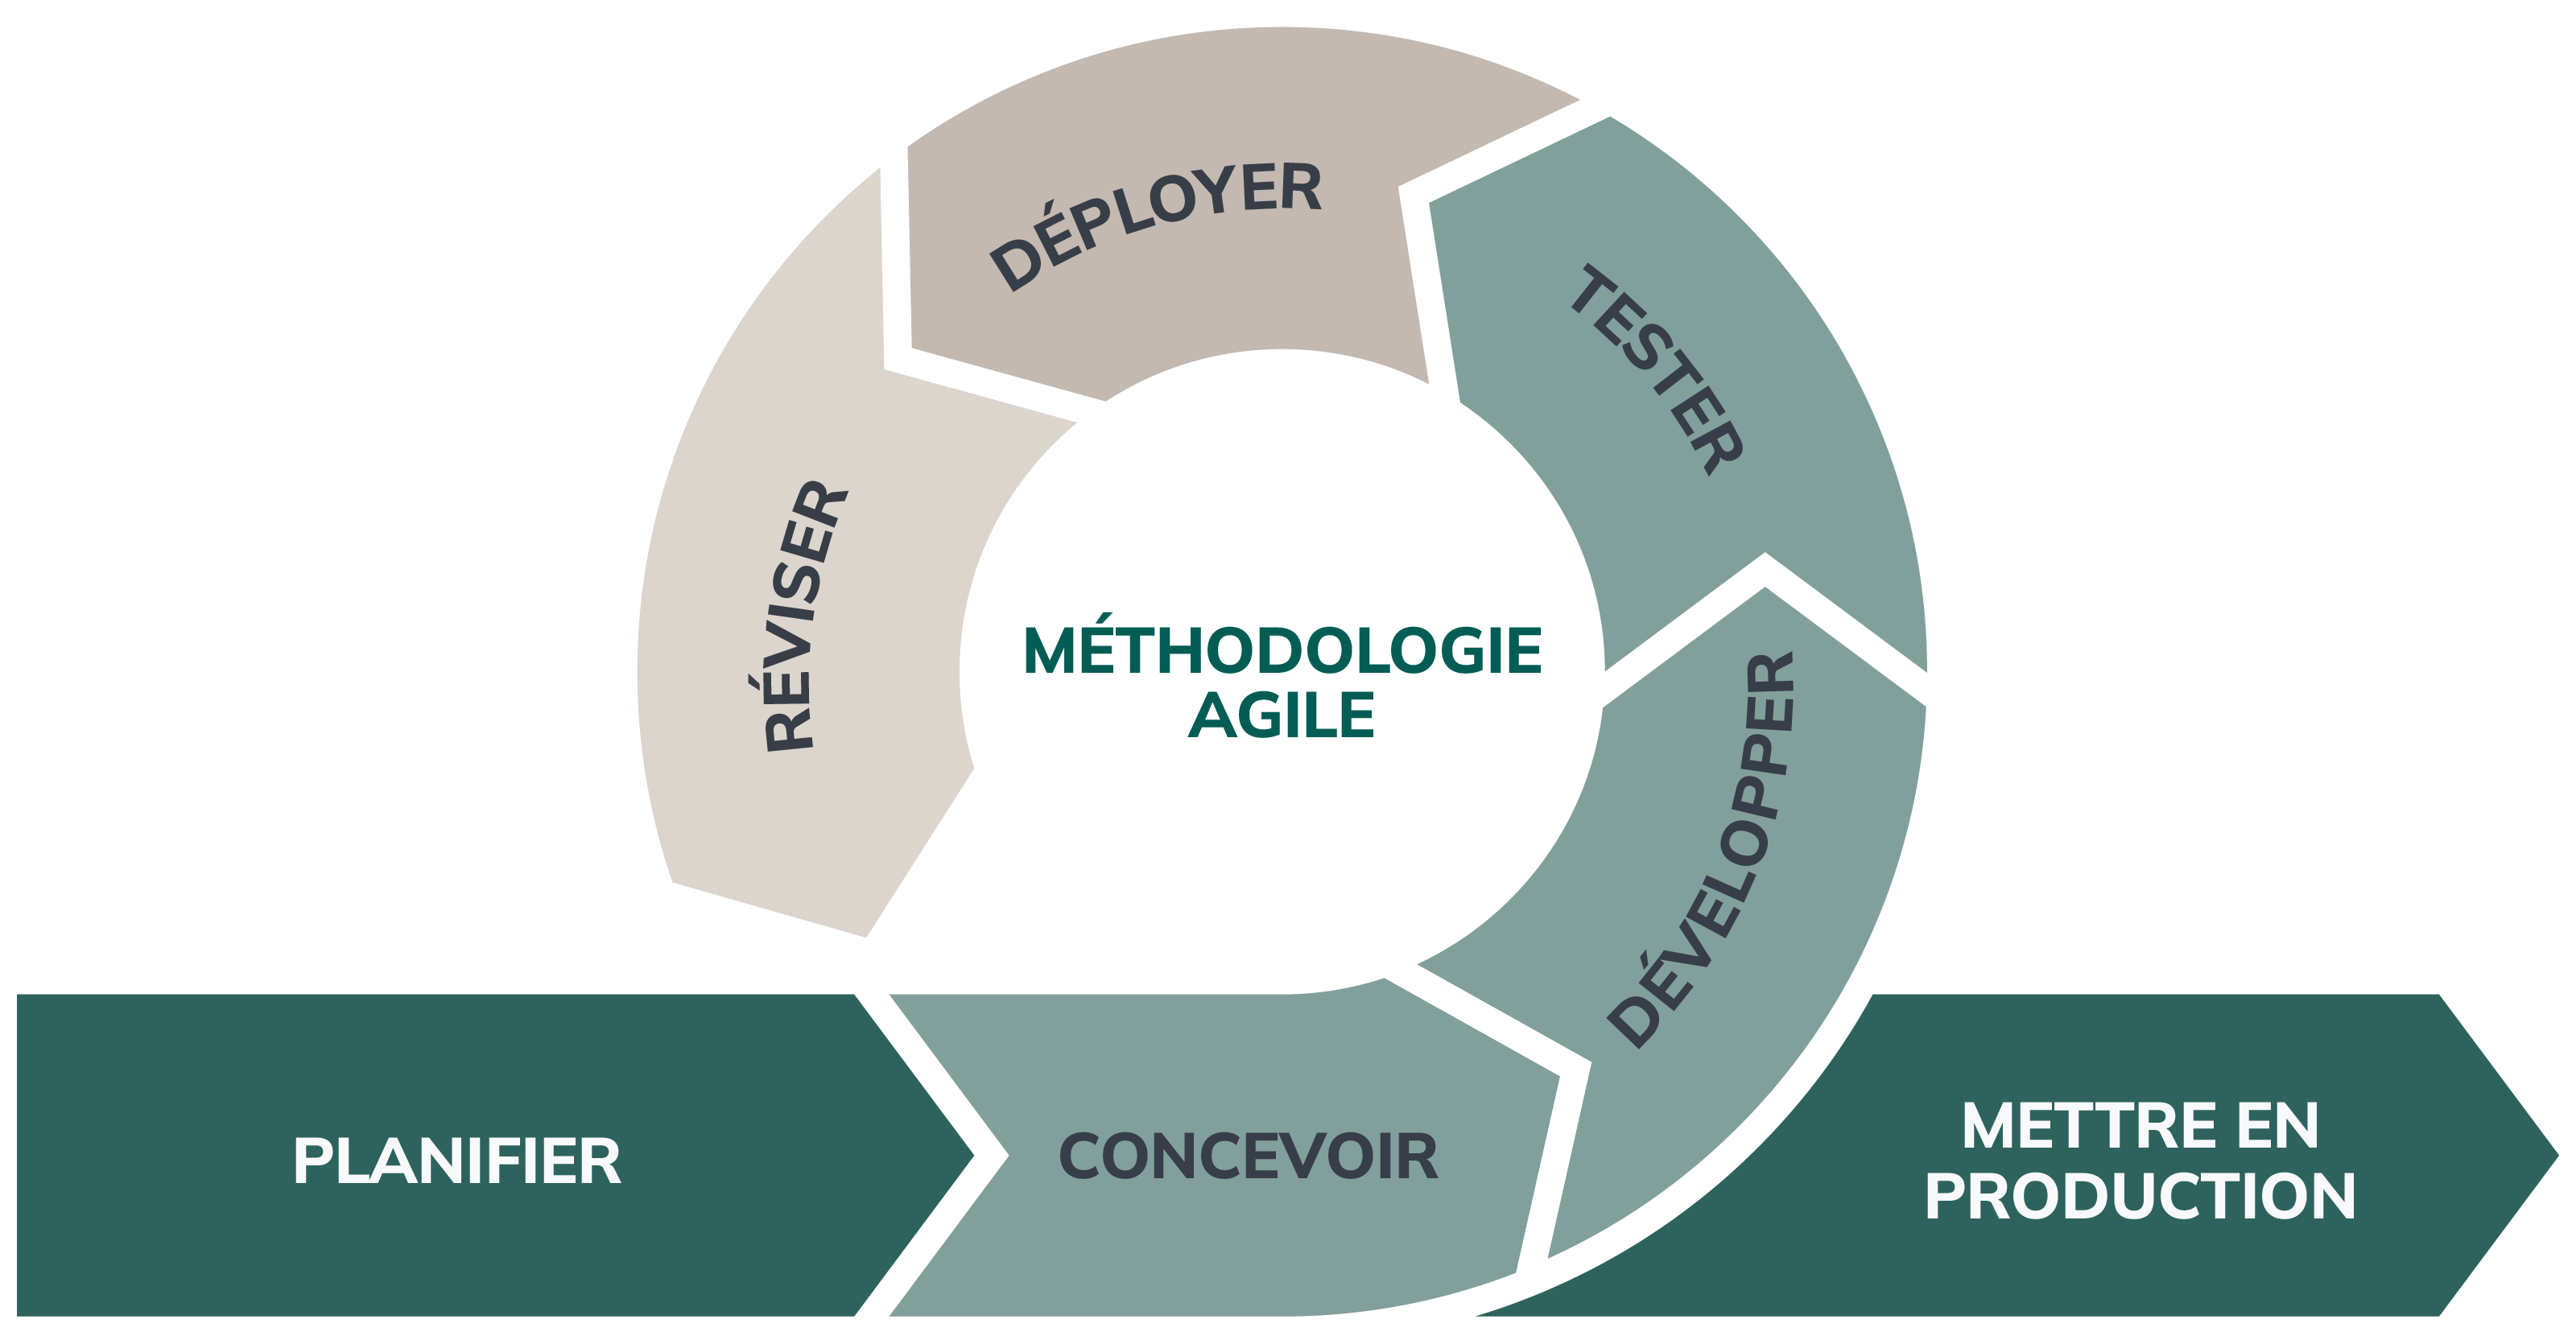
\includegraphics[width=0.8\textwidth]{figures/agile.png} % Remplace avec ton chemin d'image
    \caption{Cycle de développement Agile}
    \label{fig:agile-method}
\end{figure}

\subsection{Les principes de l’agilité}

Les principes de l’agilité mettent l’accent sur la satisfaction du client, l’adaptation au changement, la collaboration continue, et la livraison fréquente de produits fonctionnels. Ces principes sont fondamentaux dans le cadre du projet JourneyBuddy.

\subsection{Méthodologie Scrum}

La méthodologie Scrum est une mise en œuvre concrète de l’approche Agile. Elle se structure autour de rôles, d’événements, et d’artéfacts spécifiques qui organisent le travail de l’équipe de manière itérative.

\begin{figure}[H]
    \centering
    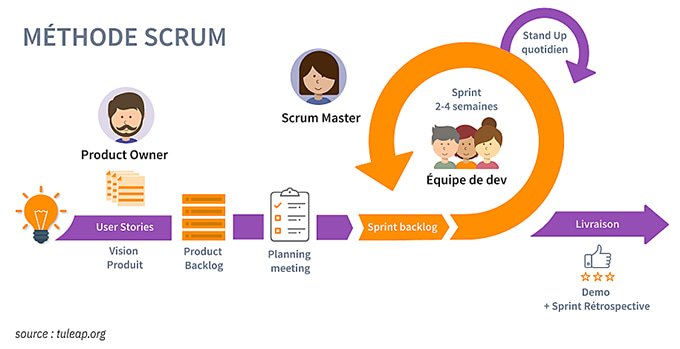
\includegraphics[width=0.8\textwidth]{figures/scrum.jpg} % Remplace avec ton chemin d'image
    \caption{Modélisation de la méthode SCRUM}
    \label{fig:scrum-method}
\end{figure}

\subsubsection{Pourquoi choisir la méthode Scrum ?}

Scrum offre une grande flexibilité, une communication continue, et une capacité à produire rapidement de la valeur tout en intégrant les retours des utilisateurs.

\textbf{Le backlog du produit}

Il s’agit d’une liste hiérarchisée de toutes les fonctionnalités souhaitées dans le produit. Elle est gérée par le Product Owner et régulièrement réévaluée.

\textbf{Les intervenants dans Scrum :}
\begin{itemize}
    \item \textbf{Product Owner} : Responsable de la définition des besoins et du backlog produit.
    \item \textbf{Scrum Master} : Garant du bon respect des règles Scrum, facilite les réunions et supprime les obstacles.
    \item \textbf{Développeurs} : Conçoivent, développent et testent les fonctionnalités au sein des sprints.
\end{itemize}

\textbf{Le Sprint}

Un sprint est une période fixe, généralement de deux semaines, durant laquelle une partie du produit est développée et rendue fonctionnelle. Chaque sprint se termine par une démonstration et une rétrospective.

\subsubsection{Adaptation de la méthodologie Scrum dans le projet}

\textbf{Nos intervenants :}
\begin{itemize}
    \item \textbf{Scrum Master} : Samia Ben Ismail
    \item \textbf{Product Owner} : Amina Dgham
    \item \textbf{Développeurs} : Amira Boubaker, Amer  Akrimi
\end{itemize}

\textbf{Product Backlog :}
\begin{table}[H]
    \centering
    \begin{tabularx}{\textwidth}{|c|X|c|}
        \hline
        \textbf{PBI} & \textbf{User Story} & \textbf{Priorité} \\
        \hline
        PB1 & En tant qu’utilisateur, je veux créer un compte pour personnaliser mon expérience. & Haute \\
        \hline
        PB2 & En tant qu’utilisateur, je veux m’authentifier afin d’accéder à mon espace personnel. & Haute \\
        \hline
        PB3 & En tant qu’utilisateur, je veux consulter les points d’intérêts disponibles. & Haute \\
        \hline
        PB4 & En tant qu’utilisateur, je veux filtrer les points d’intérêts selon des critères. & Moyenne \\
        \hline
        PB5 & En tant qu’utilisateur, je veux consulter les alertes d’événements culturels internationaux. & Moyenne \\
        \hline
        PB6 & En tant qu’utilisateur, je veux chercher un point d’intérêt par lettre alphabétique. & Basse \\
        \hline
        PB7 & En tant qu’utilisateur, je veux créer une carte de voyage soit sans, soit avec assistance AI. & Haute \\
        \hline
        PB8 & En tant qu’utilisateur, je veux chercher un vol correspondant à mon départ et arrivée avec les bonnes dates. & Haute \\
        \hline
        PB9 & En tant qu’utilisateur, je veux chercher un hôtel dans la même ville d’arrivée. & Haute \\
        \hline
        PB10 & En tant qu’utilisateur, je veux choisir le type d’accompagnant pour mon voyage. & Moyenne \\
        \hline
        PB11 & En tant qu’utilisateur, je veux saisir un budget et calculer automatiquement le montant restant. & Haute \\
        \hline
        PB12 & En tant qu’utilisateur, je veux choisir l’activité la plus proche ou la filtrer par catégorie (avec assistance AI). & Moyenne \\
        \hline
        PB13 & En tant qu’utilisateur, je veux consulter les détails du voyage avant de l’enregistrer. & Haute \\
        \hline
    \end{tabularx}
\end{table}

\begin{table}[H]
    \centering
    \begin{tabularx}{\textwidth}{|c|X|c|}
        \hline
        PB14 & En tant qu’utilisateur, je veux enregistrer ma carte de voyage. & Haute \\
        \hline
        PB15 & En tant qu’utilisateur, je veux gérer ma carte de voyage & Moyenne \\
        \hline
        PB16 & En tant qu’utilisateur, je veux consulter mon historique de cartes de voyages. & Basse \\
        \hline
        PB17 & En tant qu’utilisateur, je veux ajouter un nouveau voyage soit sans, soit avec assistance AI. & Haute \\
        \hline
        PB18 & En tant qu’utilisateur, je veux visualiser la ville d’arrivée sur une carte interactive avec Google Maps. & Haute \\
        \hline
        PB19 & En tant qu’utilisateur, je veux modifier mes informations de profil (photo, téléphone, ville/pays, bio, adresse, mot de passe). & Moyenne \\
        \hline
        PB20 & En tant qu’utilisateur, je veux gérer mes favoris pour les points d’intérêts. & Moyenne \\
        \hline
        PB21 & En tant qu’utilisateur, je veux activer ou désactiver mes préférences. & Basse \\
        \hline
        PB22 & En tant qu’utilisateur, je veux changer le thème de l’application (clair/sombre). & Basse \\
        \hline
        PB23 & En tant qu’utilisateur, je veux me déconnecter de l’application. & Haute \\
        \hline
    \end{tabularx}
    \caption{Product Backlog de JourneyBuddy}
\end{table}

\textbf{Les Sprints :}
Chaque sprint est planifié selon la priorité du backlog, et vise une livraison incrémentale d’un produit utilisable.

\begin{figure}[H]
    \centering
    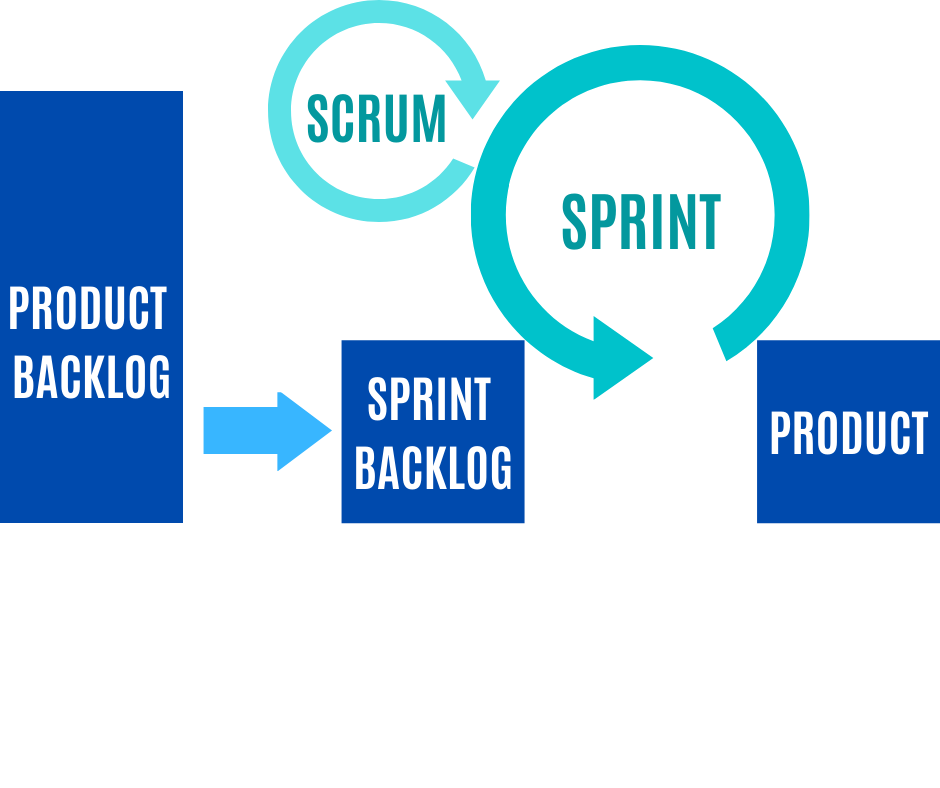
\includegraphics[width=0.7\textwidth]{figures/scrum-sprint.png} % Remplace avec ton image réelle
    \caption{Cycle de vie d’un Sprint Scrum}
    \label{fig:sprint-cycle}
\end{figure}

\begin{table}[H]
    \centering
    \begin{tabular}{|c|c|}
        \hline
        \textbf{Numéro de Sprint} & \textbf{Nom du Sprint} \\
        \hline
        Sprint 1 & Création du compte et Authentification \\
        \hline
        Sprint 2 & Planification de voyage et carte interactive \\
        \hline
        Sprint 3 & Suggestions IA et Chatbot intelligent \\
        \hline
        Sprint 4 & Finalisation UX/UI et Intégration Docker \\
        \hline
    \end{tabular}
    \caption{Découpage des Sprints pour JourneyBuddy}
    \label{tab:sprints}
\end{table}

\section{Conclusion}

Cette étude préliminaire met en lumière le potentiel de JourneyBuddy pour réinventer la planification de voyage. En se basant sur l’intelligence artificielle et une architecture agile, l’application promet une expérience personnalisée, fluide et réactive.

L’analyse du marché révèle des lacunes importantes que JourneyBuddy est capable de combler : personnalisation poussée, gestion intelligente des imprévus, et interface conversationnelle.

Grâce aux compétences techniques de l’équipe Mobelite, à son expertise en développement mobile et à l’application rigoureuse de la méthodologie SCRUM, le projet est bien positionné pour répondre aux attentes du marché.

\textbf{Prochaines étapes :}
\begin{itemize}
    \item Rédaction des spécifications techniques.
    \item Optimisation de l’expérience utilisateur.
    \item Lancement du prototype et itérations selon les retours utilisateurs.
\end{itemize}

JourneyBuddy ambitionne ainsi de devenir un compagnon de voyage incontournable dans l’ère numérique.
